\documentclass[tikz,border=5mm]{standalone}
\usetikzlibrary{decorations.pathmorphing, arrows.meta,bending}

\begin{document}
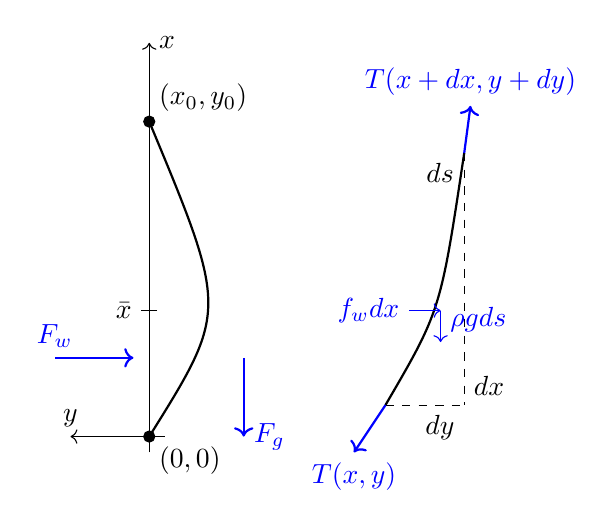
\begin{tikzpicture}[scale=2]
  \coordinate (A) at (0,2);  % Adjust x_0 as needed
  \coordinate (B) at (0,0);
  \coordinate (C) at (0.5,0.8);

  % Cable curve (adjust control points for finer tuning)
  \draw[thick, black] (A) .. controls (C) .. (B);

  % Axes
  \draw[->, black] (0, -0.1) -- (0, 2.5) node[right] {$x$};
  \draw[->, black] (0.1, 0) -- (-0.5,0) node[above] {$y$};
  % xbar
  \draw (0.05, 0.8) -- (-0.05, 0.8) node[left] {$\bar{x}$};

  % Label points
  \filldraw (A) circle (1pt) node[above right] {$(x_0, y_0)$};
  \filldraw (B) circle (1pt) node[below right] {$(0, 0)$};

  % Forces
  \draw[->, thick, blue] (0.6, 0.5) -- (0.6, 0) node[right] {$F_g$};
  \draw[<-, thick, blue] (-0.1, 0.5) -- (-0.6, 0.5) node[above] {$F_w$};

  % small segment
  \coordinate (D) at (1.5, 0.2);
  \coordinate (E) at (2.0, 1.8);
  \coordinate (F) at (1.85, 0.8);
  \draw[thick, black] (D) .. controls (F) .. (E) node[below left] {$ds$};
  \draw[dashed, black] (D) -- ++(0.5, 0) node[below left] {$dy$};
  \draw[dashed, black] (E) -- ++(0, -1.6) node[above right] {$dx$};
  \draw[->, thick, blue] (D) -- ++(-0.2, -0.3) node[below] {$T(x,y)$};
  \draw[->, thick, blue] (E) -- ++(0.04, 0.3) node[above] {$T(x+dx,y+dy)$};
  \draw[->, blue] (F) -- ++(0, -0.2) node[above right] {$\rho g ds$};
  \draw[<-, blue] (F) -- ++(-0.2, 0) node[left] {$f_w dx$};

\end{tikzpicture}
\end{document}
